%
% Portuguese-BR vertion
% 
\documentclass{article}

\usepackage{hsm_tb}
% Use longtable if you want big tables to split over multiple pages.
% \usepackage{longtable}
\usepackage[utf8]{inputenc} 
\usepackage[spanish]{babel} % Uncomment for portuguese

\sloppy

\graphicspath{{./pictures/}} % Pictures dir
\makeindex
\begin{document}

\DocumentTitle{Documento de Pruebas de Proyecto}
\Project{Módulo hardware de criptografía ligera orientado al internet de las cosas}
\Organization{CIATEQ}
\Version{Versión 1.0a}

\capa
\newpage

%%%%%%%%%%%%%%%%%%%%%%%%%%%%%%%%%%%%%%%%%%%%%%%%%%
%% Revision History
%%%%%%%%%%%%%%%%%%%%%%%%%%%%%%%%%%%%%%%%%%%%%%%%%%
\section*{\center Histórico de Revisiones}
  \vspace*{1cm}
  \begin{table}[ht]
    \centering
    \begin{tabular}[pos]{|m{2cm} | m{7.2cm} | m{3.8cm}|} 
      \hline
      \cellcolor[gray]{0.9}
      \textbf{Date} & \cellcolor[gray]{0.9}\textbf{Descripción} & \cellcolor[gray]{0.9}\textbf{Autor(es)}\\ \hline
      \hline
      \small xx/xx/xxxx & \small <Descripción> & \small <Autor(es)> \\ \hline      
      \small xx/xx/xxxx &
      \begin{small}
        \begin{itemize}
          \item item;
          \item item;
        \end{itemize}
      \end{small} & \small <Autor(es)> \\ \hline 
    \end{tabular}
  \end{table}

\newpage

% TOC instantiation
\tableofcontents
\newpage

%%%%%%%%%%%%%%%%%%%%%%%%%%%%%%%%%%%%%%%%%%%%%%%%%%
%% Document main content
%%%%%%%%%%%%%%%%%%%%%%%%%%%%%%%%%%%%%%%%%%%%%%%%%%
\section{Introducción}

\subsection{Vista Geral del Documento}
En este documento se redacta la información necesaria para realizar las pruebas al módulo hardware para seguridad basado en el estándar~\cite{1059-1993-std:1994}.

  \begin{itemize}
   \item \textbf{Requisitos funcionales -} Lista de todos los requisitos funcionales.
   \item \textbf{Requisitos no funcionales -} Lista de todos los requisitos no Funcionales.
   \item \textbf{Dependencias -} Conjunto de dependencias de IP-cores previstos.
   \item \textbf{Notas -} Lista de notas presentadas en el documento.
   \item \textbf{Referencias -} Lista de todos los textos referenciados en el documento.
  \end{itemize}

  % inicio das definições do documento
  \subsection{Definiciones}
    \FloatBarrier
    \begin{table}[H]
      \begin{center}
        \begin{tabular}[pos]{|m{5cm} | m{9cm}|} 
          \hline
          \cellcolor[gray]{0.9}\textbf{Término} & \cellcolor[gray]{0.9}\textbf{Descripción} \\ \hline
          Requisitos Funcionales & Requisitos que hacen funcional al sistema, son las capacidades que debe tener el sistema entregado.  \\ \hline
					Requisitos Técnicos & Requisitos del sistema que definen características referentes a técnicas, algoritmos, tecnologías y especificidades de los requerimientos funcionales.  \\ \hline
          Requisitos No Funcionales & Requisitos de los módulos entregables.  Se refieren a las capacidades no funcionales del sistema como un todo y que especifican necesidades del usuario final.  \\ \hline
          Dependencias & Requisitos de reuso de IP-cores, describiendo las funciones que cada uno de estos módulos debe realizar. \\ \hline
        \end{tabular}
      \end{center}
    \end{table}  
  % fim

  % inicio da tabela de acronimos e abreviacoes do documento
  \subsection{Acrónimos y abreviaciones}
    \FloatBarrier
    \begin{table}[H]
      \begin{center}
        \begin{tabular}[pos]{|m{2cm} | m{12cm}|} 
          \hline
          \cellcolor[gray]{0.9}\textbf{Sigla} & \cellcolor[gray]{0.9}\textbf{Descripción} \\ \hline
          FR      & Requisito Funcional  \\ \hline
					TR      & Requisito Técnico  \\ \hline
          NFR     & Requisito No Funcional  \\ \hline
          D       & Dependencia  \\ \hline
        \end{tabular}
      \end{center}
    \end{table}  
  % fim

  % inicio da descriao de prioridades de requisitos
  \subsection{Prioridades de los Requisitos}
    \FloatBarrier
    \begin{table}[H]
      \begin{center}
        \begin{tabular}[pos]{|m{2cm} | m{12cm}|} 
          \hline
          \cellcolor[gray]{0.9}\textbf{Prioridad} & \cellcolor[gray]{0.9}\textbf{Característica} \\ \hline
          Importante     & Requisito para que el sistema sea entregado.  \\ \hline
          Esencial       & Requisito que debe ser implementado para que el sistema funcione.  \\ \hline
          Deseable       & Requisito que no compromete el funcionamento del sistema.  \\ \hline
        \end{tabular}
      \end{center}
    \end{table}  
  % fim

  % inicio dos requisitos Funcionales
  \section{Requisitos Funcionales}
	
En un sistema HSM, un controlador maestro envía peticiones de servicios continuamente al HSM, entonces, el HSM responde a dichas peticiones con servicios de seguridad. Debido a que hay muchas solicitudes del controlador maestro, el HSM debe responder a las solicitudes muy rápidamente. Para este propósito, el microcontrolador y otros módulos FPGA deben estar altamente optimizados~\cite{evita-hsm:2012}. 

En esta etapa del desarrollo del HSM, no se determina cómo tomará forma el progreso del software que utilizará los servicios del HSM, los requisitos existentes definen las funcionalidades del sistema y los algoritmos que se implementarán en FPGA para el cifrado, el \textit{hashing}, firma digital y la generación de llaves.

    \subsection{Requisitos Funcionales}
    \begin{functional}
     % format \requirement{name}{description}{priority}
     \requirement{fr1}
		  {Cada llave debe ser usada por una sola función criptográfica}
      {The HSM ensures that each cryptographic key is only used for a single cryptographic function and only for its intended purpose.}
      {Importante}
    
     \requirement{fr2}
		  {Cálculo de resumen (\textit{hash}) de mensajes}
      {permite la generación y verificación firmas digitales hash y adicionalmente HMAC.}
      {Importante}
			
     \requirement{fr3}
      {Cifrador asimétrico}
      {Descripción breve y objetiva.}
      {Importante}
			
     \requirement{fr4}
      {Cifrador simétrico}
      {Descripción breve y objetiva.}
      {Importante}
			
     \requirement{fr5}
      {Cálculo de números pseudo-aleatorios}
      {Descripción breve y objetiva.}
      {Importante}
			
			\requirement{fr6}
			{Proveer un contador monotónico}
			{Descripción breve y objetiva.}
			{Importante}
			
			\requirement{fr7}
			{Creación de llaves internamente}
			{Descripción breve y objetiva.}
			{Importante}
			
    \end{functional}

  \subsection{Requisitos Técnicos de los Requisitos Funcionales}
  
    \begin{technical}
      \techrequirement
			{Requisitos Técnicos de FR\ref{fr1}}
			{
      \begin{itemize}
        \item[$-$]{Los datos que serán utilizados llegan bloque a bloque al HSM}
        \item[$-$]{El algoritmo utilizado es SHA-256}
				\item[$-$]{El \textit{hash} se envía a una dirección especificada previamente}
      \end{itemize}
      }
			
      \techrequirement
			{Requisitos Técnicos de FR\ref{fr2}}
      {
      \begin{itemize}
        \item[$-$]{Los datos que serán utilizados llegan bloque a bloque al HSM}
        \item[$-$]{El algoritmo utilizado es SHA-256}
				\item[$-$]{El \textit{hash} se envía a una dirección especificada previamente}
      \end{itemize}
      }
			
			\techrequirement
			{Requisitos Técnicos de FR\ref{fr3}}
      {
      \begin{itemize}
        \item[$-$]{El algoritmo utilizado es AES-128}
      \end{itemize}
      }
			
			\techrequirement
			{Requisitos Técnicos de FR\ref{fr4}}
      {
      \begin{itemize}
        \item[$-$]{Los datos que serán utilizados llegan bloque a bloque al HSM}
        \item[$-$]{El algoritmo utilizado es SHA-256}
				\item[$-$]{El \textit{hash} se envía a una dirección especificada previamente}
      \end{itemize}
      }
			
			\techrequirement
			{Requisitos Técnicos de FR\ref{fr5}}
      {
      \begin{itemize}
        \item[$-$]{Los datos que serán utilizados llegan bloque a bloque al HSM}
        \item[$-$]{El algoritmo utilizado es SHA-256}
				\item[$-$]{El \textit{hash} se envía a una dirección especificada previamente}
      \end{itemize}
      }
			
			\techrequirement
			{Requisitos Técnicos de FR\ref{fr6}}
      {
      \begin{itemize}
        \item[$-$]{Los datos que serán utilizados llegan bloque a bloque al HSM}
        \item[$-$]{El algoritmo utilizado es SHA-256}
				\item[$-$]{El \textit{hash} se envía a una dirección especificada previamente}
      \end{itemize}
      }
			
			\techrequirement
			{Requisitos Técnicos de FR\ref{fr7}}
      {
      \begin{itemize}
        \item[$-$]{Los datos que serán utilizados llegan bloque a bloque al HSM}
        \item[$-$]{El algoritmo utilizado es SHA-256}
				\item[$-$]{El \textit{hash} se envía a una dirección especificada previamente}
      \end{itemize}
      }
    \end{technical}    
 
\section{Requisitos no Funcionales}
% Esta seção apresenta a lista de Requisitos No Funcionales do projeto.

  \begin{nonfunctional}
    \requirement{nfr1}
		{Nombre del Requisito}
    {Descripción breve y objetiva.}
    {Importante}

    \requirement{nfr2}
		{Nombre del Requisito}
    {Descripción breve y objetiva.}
    {Importante}
  \end{nonfunctional}

\section{Dependencias}
  % Esta seção apresenta uma lista dos IP-cores disponíveis % para reuso e que devem ser adotados no desenvolvimento % deste projeto.

  \begin{dependencies}
    \dependency{Nombre del IP-\textit{core}}
		{Descripción breve y objetiva del IP-\textit{core} y referencia al documento.}

    \dependency{Nombre del IP-\textit{core}}
		{Descripción breve y objetiva del IP-\textit{core} y referencia al documento.}
  \end{dependencies}  

\section{Análisis estático con herramientas Lint}

 What Verilator Does
Verilator is invoked with parameters similar to GCC or Synopsys’s VCS. It "Verilates" the specified synthesizable Verilog or SystemVerilog code by reading it, performing lint checks, and optionally inserting assertion checks and coverage-analysis points. It outputs single- or multi-threaded .cpp and .h files, the "Verilated" code.

The user writes a little C++/SystemC wrapper file, which instantiates the "Verilated" model of the user’s top level module. These C++/SystemC files are then compiled by a C++ compiler (gcc/clang/MSVC++). The resulting executable performs the design simulation. Verilator also supports linking its generated libraries, optionally encrypted, into other simulators.

Verilator may not be the best choice if you are expecting a full featured replacement for NC-Verilog, VCS or another commercial Verilog simulator, or if you are looking for a behavioral Verilog simulator e.g. for a quick class project (we recommend Icarus Verilog for this.) However, if you are looking for a path to migrate synthesizable Verilog to C++ or SystemC, and your team is comfortable writing just a touch of C++ code, Verilator is the tool for you.

go to https://www.veripool.org/projects/verilator/wiki/Installing

  \begin{figure}[h]
    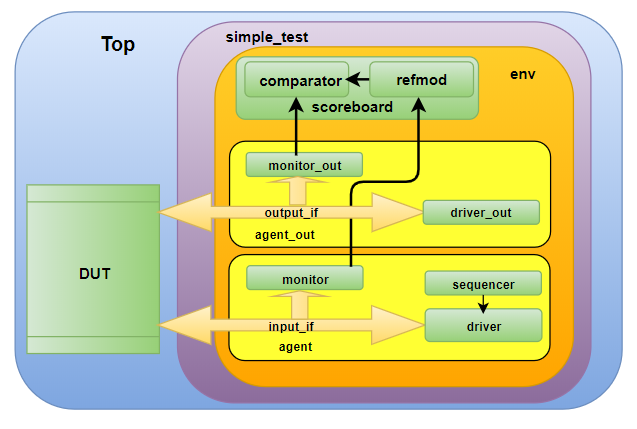
\includegraphics[width=0.6\linewidth]{pictures/uvm.png}
    \label{uvm_tb}
  \end{figure}
		
% Optional bibliography section
% To use bibliograpy, first provide the ipprocess.bib file on the root folder.
\newpage
\bibliographystyle{ieeetr}
\bibliography{bibliography}

\end{document}